\documentclass[11pt]{article}
\usepackage[T1]{fontenc}
\usepackage[a4paper,margin=1in]{geometry}
\usepackage{amsmath,amssymb,amsthm}
\usepackage{mathrsfs}
\usepackage{graphicx}
\usepackage[hidelinks]{hyperref}
\usepackage{microtype}

\newtheorem*{question}{Source question}
\newtheorem*{answer}{Burguet--Shi main theorem}

\setlength{\parindent}{0pt}
\setlength{\parskip}{0.58em}

\title{Literature Status: Positive Entropy Forces Infinite\\
Mean Dimension on the Space of Measures}
\author{Run \texttt{fa\_banach\_001} --- lane 1}
\date{13 August 2026}

\begin{document}
\maketitle

\begin{center}
\fbox{\parbox{0.9\textwidth}{
\textbf{Status: literature already answered (fully, and more strongly).}
The open question in arXiv:1105.0360 asks whether positive entropy of a
continuous self-map forces positive topological mean dimension of its
push-forward action on probability measures.  The main theorem of
Burguet and Shi, arXiv:2206.10508, proves that this induced mean dimension
is in fact infinite for every positive-entropy compact dynamical system.
}}
\end{center}

\section{The source question}

B. Kloeckner, \emph{A generalization of Hausdorff dimension applied to
Hilbert cubes and Wasserstein spaces}, arXiv:1105.0360, proves that if
$X$ is compact and $\varphi:X\to X$ has positive topological entropy,
then the induced push-forward map $\varphi_\#$ on the Wasserstein space
$\mathscr W_p(X)$ has positive \emph{metric} mean dimension.  Directly
after Corollary~1.3, the paper asks~\cite{source}:

\begin{question}
Is the (topological) mean dimension of $\varphi_\#$ positive whenever
$\varphi$ has positive entropy?  The source notes that determining this
even for one map $\varphi$ would be interesting.
\end{question}

Here $\mathscr W_p(X)$ is the space of Borel probability measures on the
compact metric space $X$, equipped with a Wasserstein metric.

\section{The later theorem}

D. Burguet and R. Shi, \emph{Topological mean dimension of induced
systems}, arXiv:2206.10508, consider the same induced system.  They write
$\mathcal M(X)$ for the Borel probability measures on $X$ with the
weak-* topology and $T_*\mu=\mu\circ T^{-1}$.  Their main theorem
states~\cite{answerpaper}:

\begin{answer}
For any topological system $(X,T)$ with positive topological entropy,
the induced system $(\mathcal M(X),T_*)$ has infinite topological mean
dimension.  Equivalently,
\[
 h_{\mathrm{top}}(T)>0
 \quad\Longleftrightarrow\quad
 \operatorname{mdim}(T_*)>0
 \quad\Longleftrightarrow\quad
 \operatorname{mdim}(T_*)=\infty.
\]
\end{answer}

For compact $X$, every finite-order Wasserstein metric induces the
weak-* topology on the probability measures.  Thus the topological
dynamical systems denoted by $(\mathscr W_p(X),\varphi_\#)$ in the source
and $(\mathcal M(X),T_*)$ in the later paper are the same after setting
$T=\varphi$.  The later theorem therefore answers the exact source
question for every positive-entropy map, and strengthens ``positive'' to
``infinite.''

No new mathematical result is claimed in this packet.

\clearpage
\section{Primary-source evidence}

The following crop is from arXiv:1105.0360, PDF page~5.  It contains
Corollary~1.3 and the ensuing open question.

\begin{center}

\includegraphics[width=0.96\textwidth]{figures/source_question_crop.png}
\end{center}

The following crop is from arXiv:2206.10508, PDF page~1.  It records the
definition of the induced system and the main theorem.

\begin{center}
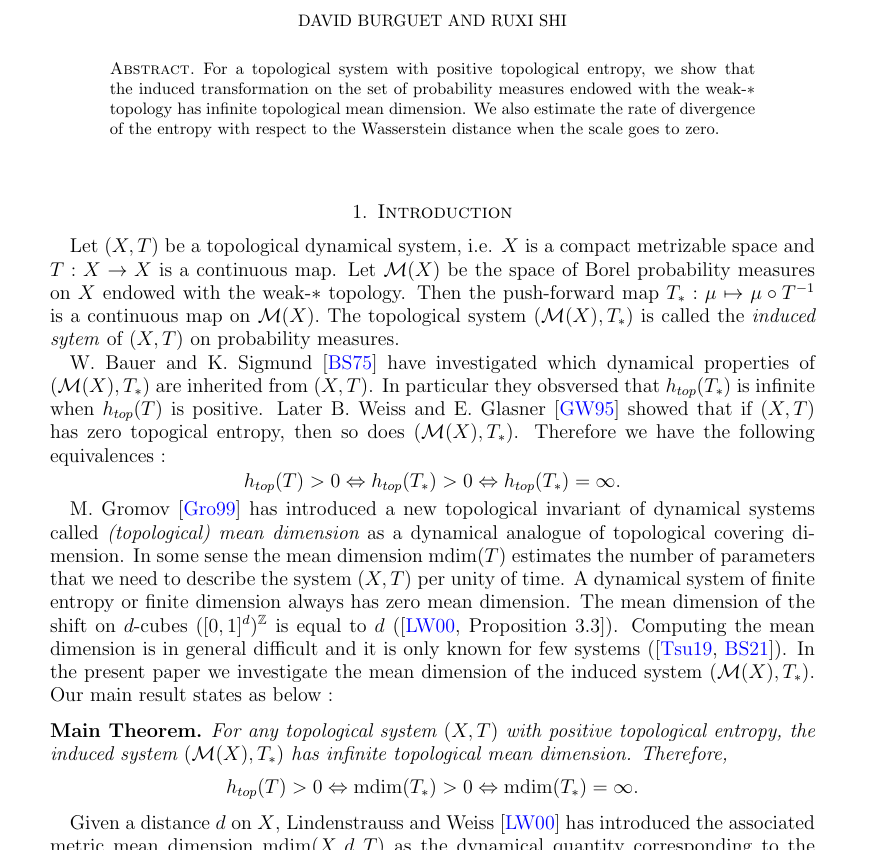
\includegraphics[width=0.96\textwidth]{figures/later_theorem_crop.png}
\end{center}

\begin{thebibliography}{9}
\bibitem{source}
B. Kloeckner,
\emph{A generalization of Hausdorff dimension applied to Hilbert cubes
and Wasserstein spaces}, arXiv:1105.0360 (2011).

\bibitem{answerpaper}
D. Burguet and R. Shi,
\emph{Topological mean dimension of induced systems},
arXiv:2206.10508 (2022).
\end{thebibliography}

\end{document}
